\chapter{Fundamentação Teórica}

A sinalização semafórica pode ser feita com uma de duas funções planejadas: a de regulamentar o direito de passagem de fluxos de veículos e pedestres nas vias, ou de advertir os condutores de veículos e pedestres sobre obstáculos ou situações perigosas nas vias. A composição da sinalização semafórica é um conjunto de indicações luminosas, acionadas alternadamente ou intermitentemente, fixado em posições, próximas à via, que as tornem fáceis de identificar e interpretar para condutores e pedestres. 
%[http://meusite.mackenzie.br/professor_cucci/ManualSemaforos2014.pdf]

A tabela \ref{tab: focos} mostra as definições de formas e dimensões da sinalização semafórica a ser utilizada, dependendo de sua finalidade.

\begin{table}[H]
\centering
\caption{Definições de formas e dimensões}
\label{tab: focos}
\begin{tabular}{@{}lllll@{}}
\toprule
Semáforos destinados a & Forma do foco & Dimensão da lente (mm) \\ \midrule
Veículos automotores & Circular & Diâmetro de 200 ou 300 \\
Bicicletas & Circular & Diâmetro de 200 ou 300 \\
Faixas reversíveis          &	Quadrada & Lado de 300		  \\
Advertência & Circular & Diâmetro de 200 ou 300 \\
Pedestres & Quadrada & Lado de 200 ou 300 \\
\bottomrule
\end{tabular}
\end{table}
% http://meusite.mackenzie.br/professor_cucci/ManualSemaforos2014.pdf

A maneira mais eficiente de realizar o controle de sinalização semafórica, controlando e temporizando o acendimento alternado das indicações luminosas é dada utilizando circuitos eletrônicos, feitos especificamente para essa finalidade. A esse sistema dá-se o nome de sistema embarcado. 

\section{Sistemas embarcados}

%\subsection{LED}

Um sistema embarcado pode ser entendido como uma combinação de hardware (placas de circuito impresso, circuitos integrados, componentes eletrônicos) e software (programação carregada em processadores), que é feito para um fim específico e pré-determinado, sendo assim bastante confiável e otimizado, e possibilitando menor custo nos projetos (um sistema feito para funções generalizadas costuma custar mais caro). A interação com o ambiente externo se dá por meio de sensores e atuadores, apresentando uma interface simplificada, dependendo da utilização, como botões de on/off e LEDs de sinalização. 
%[Michael Barr. Programming Embedded Systems in C and C++. cap1]

\begin{figure}[ht]
    \begin{center}
    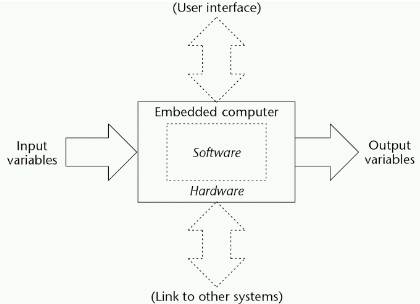
\includegraphics{figuras/embedded.PNG}
    \end{center}
    \caption[]{Visão geral da integração de um sistema embarcado}
    \label{embarcado}
\end{figure}
%[http://www.eletrica.ufpr.br/mehl/te200/aulas/embarcados.pdf]

O avanço da tecnologia, porém, permitiu a confecção de sistemas cada vez mais elaborados e capazes, fazendo com que os sistemas embarcados se tornem cada vez mais abrangentes, contradizendo a definição de sistema feito para fins específicos. Para utilização de sistemas embarcados em seus projetos, um projetista deve estudar os requisitos de tal projeto, escolher o hardware específico para a realização das tarefas e, por fim, escrever um software otimizado para o circuito montado. %[http://www.eletrica.ufpr.br/mehl/te200/aulas/embarcados.pdf].

Sistemas embarcados podem ser encontrados em diversos dispositivos do dia a dia, realizando diferentes tipos de controle, e em alguns casos, agindo em conjunto com outros sistemas embarcados, compondo um sistema maior e completo.
Um sistema embarcado necessita de um núcleo de processamento para realizar as tarefas necessárias, chamado de processador. Além disso, necessita também de circuitos periféricos que permitam que o processador se comunique com o meio externo. Dá-se o nome de microcontrolador, ao conjunto de um processador com tais periféricos, em um único chip.      
O foco deste trabalho é falar sobre a utilização de microcontroladores como solução para controle de sinalização semafórica. 

\subsection{Microprocessadores}

Os processadores são a unidade central de um sistema embarcado que processa dados e instruções, eles realizam as tarefas e controlam o funcionamento dos periféricos, funcionam com um clock, recebem dados binários como entrada, armazenando-os em registradores, e realizam operações com tais dados, enviando o resultado como saída. 
%[Osborne, Adam (1980). An Introduction to Microcomputers. Volume 1: Basic Concepts (2nd ed.). Berkeley, California: Osborne-McGraw Hill.]

O primeiro processador disponível no mercado foi o Intel 4004, lançado em 1971, com uma capacidade de processamento de 4 bits, velocidade de clock de 750 KHz,  interface para interagir com memórias RAM, ROM e um canal digital de 4 bits de comunicação de entrada e saída 
%[http://www.intel4004.com/The_MOS_Silicon_Gate_Technology_and_the_First_Microprocessors.pdf em http://www.intel4004.com/]

\begin{figure}[ht]
    \begin{center}
    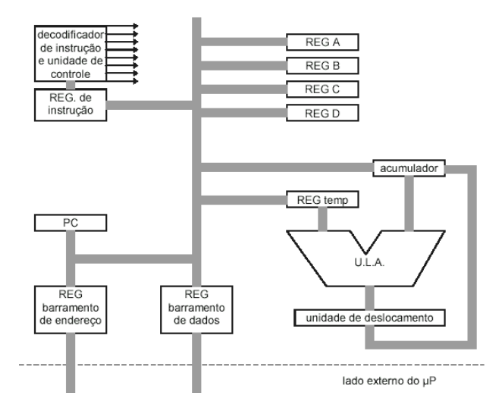
\includegraphics{figuras/processor.PNG}
    \end{center}
    \caption[Sistema embarcado]{Visão geral da integração de um sistema embarcado.}
    \label{processor}
\end{figure}

%[http://iris.sel.eesc.usp.br/sel433a/Micros.pdf]

A Figura \ref{processor} Apresenta de modo simplificado a estrutura interna de um microprocessador, onde pode-se notar os registradores, que são armazenadores de dados, e suas duas unidades básicas: a unidade lógica aritmética (ULA), onde ocorrem as operações lógicas e aritméticas, e a unidade de controle (UC), responsável pela execução das instruções %http://iris.sel.eesc.usp.br/sel433a/Micros.pdf
Os processadores possuem parâmetros que definem o modo e a velocidade de operação dos mesmos, que serão explicados a seguir.

\subsubsection{Capacidade de processamento}

A capacidade de processamento, com a qual um processador consegue trabalhar, representa o número de bits que pode ser processado por instrução, também chamado de palavra. Uma instrução é definida como uma única ação que o processador pode executar por vez %http://iris.sel.eesc.usp.br/sel433a/Micros.pdf 
Um processador com capacidade de processamento de 4 bits, por exemplo, consegue processar dados de até 4 bits (equivalente a 24, ou 16) por vez. Com o avanço da tecnologia, a capacidade dos processadores foi aumentando drasticamente, sendo encontrados, hoje, nos microcontroladores no mercado, dispositivos com capacidades que variam entre 8, 16 e 32 bits (28 = 256; 216 = 65536; 232 = 4294967296).

\subsubsection{Velocidade de Clock}

Frequência do clock. Quantidade de ciclos por segundo. Além disso, existe a quantidade de instruções por segundo. A velocidade do clock de um processador determina o quão rápido ele consegue realizar as suas instruções. O intel 4004 tinha um clock máximo de 740 kHz, que equivale a 740 mil pulsos por segundo. Os microprocessadores atuais alcançam velocidades acima de 500 Mhz (mais de 650 vezes mais rápidos). 

Além da velocidade de clock, os processadores possuem um parâmetro que determina quantos ciclos desse clock são necessários para que uma instrução seja realizada. O Intel 4004 necessitava de 8 ciclos por instrução, enquanto alguns microprocessadores modernos conseguem realizar 945 MIPS (milhões de instruções por segundos) com um clock de 600 MHz (resultando em mais de 1.5 instruções por ciclo de clock) %[http://ww1.microchip.com/downloads/en/DeviceDoc/60001525A.pdf]

\begin{figure}[ht]
    \begin{center}
    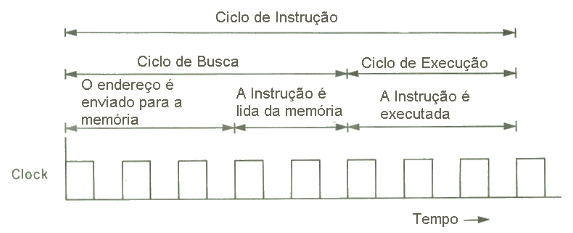
\includegraphics{figuras/clock.PNG}
    \end{center}
    \caption[Sequencia de instrução]{Processo de execução de instrução do processador.}
    \label{clock}
\end{figure}

A Figura \ref{clock} mostra o comportamento do sinal de clock, e as atividades realizadas, durante o mesmo, pelo microprocessador para realizar uma instrução.

\subsubsection{Periféricos}

Mesmo sendo o núcleo computacional do sistema, um microprocessador não seria de grande utilidade, sem a integração com elementos externos, como memórias, para armazenamento de dados, e canais de entrada e saída de dados (chamados de portas I/O). A maneira mais simplificada de integrar os periféricos ao microprocessador, como foi integrado o Intel 4004, é utilizando uma memória RAM, uma memória ROM e um canal de portas I/O (no caso do 4004, era um canal de 4 bits).

\begin{figure}[ht]
    \begin{center}
    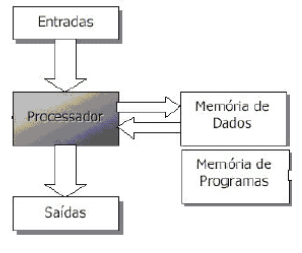
\includegraphics{figuras/processor_periph.PNG}
    \end{center}
    \caption[Periféricos do processador]{Interação do processador com as memórias.}
    \label{perifericos}
\end{figure}

%http://iris.sel.eesc.usp.br/sel433a/Micros.pdf

%\begin{labeling}{17.5.3.3}
%    \item[17.5.3] Em todos os locais de trabalho deve haver iluminação adequada, natural ou artificial, geral ou suplementar, apropriada à natureza da atividade.
%    \item[17.5.3.1]  A iluminação geral deve ser uniformemente distribuída e difusa.
%   \item[17.5.3.2] A iluminação geral ou suplementar deve ser projetada e instalada de forma a evitar ofuscamento, reflexos incômodos, sombras e contrastes excessivos.
%    \item[17.5.3.3] Os níveis mínimos de iluminamento a serem observados nos locais de trabalho são os valores de iluminâncias estabelecidos na NBR 5413, norma brasileira registrada no INMETRO.
%\end{labeling}

A memória RAM (memória de acesso aleatório) é utilizada pelo microprocessador para armazenar e ler dados. Por se tratar de uma memória volátil, os dados contidos nela são apagados quando é desenergizada.
Já a memória ROM (memória apenas de leitura) é utilizada para armazenar as instruções a serem executadas pelo microprocessador. Por se tratar de uma memória não volátil, os dados salvos nela não são apagados quando o sistema é desenergizado, garantindo que o programa gravado seja sempre executado ao ligar o microprocessador. Apesar do nome, existem variantes dessa memória que permitem a regravação de dados (EPROM, EEPROM).

Com as memórias, o microprocessador pode executar instruções salvar dados, porém ainda é necessário um canal de comunicação com o meio externo, que é satisfeito com a integração de um canal de comunicação com entrada e saída (I/O) de dados digitais. Nos barramentos I/O, cada entrada, ou saída, representa um bit. 

Com esses periféricos, o microprocessador é capaz de identificar instruções, aceitar e armazenar dados vindo do ambiente externo, processar tais dados e enviar o resultado de volta ao ambiente externo. Outros periféricos podem ser integrados, e são utilizados em microprocessadores modernos. Alguns serão explicados em outras seções desse trabalho.


\subsection{Microcontroladores}

Enquanto um microprocessador é feito para realizar tarefas genéricas, ele pode ser integrado com determinados elementos periféricos, para especificar uma finalidade de uso. Quando essa combinação de dispositivos é disposta em um único chip, dá-se o nome de microcontrolador.

Um microcontrolador, de maneira simplificada, é composto de um processador, em conjunto com memórias RAM e ROM e um canal de entrada e saída de dados (interface I/O), tendo outras funcionalidades, dependendo da família de produtos escolhida. Um microcontrolador é um hardware bastante versátil, podendo ser utilizado em várias aplicações que necessitem de soluções inteligentes de baixo custo, que compõe a parte do hardware envolvido no sistema embarcado. Apesar da versatilidade, quando um microcontrolador é escolhido para um projeto, suas funções passam a ser bastante específicas, por conta do circuito eletrônico que é montado em volta dele, e do software que é escrito especificamente para aquela finalidade.

\begin{figure}[ht]
    \begin{center}
    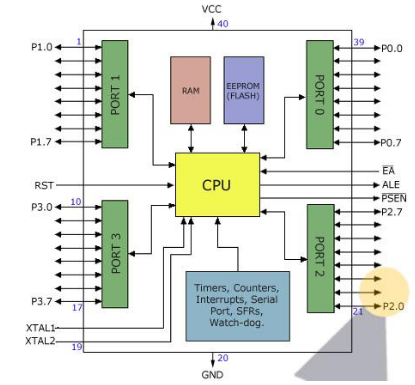
\includegraphics{figuras/microprocessador.PNG}
    \end{center}
    \caption[Microcontrolador]{Integração do processador com periféricos.}
    \label{microcontrolador}
\end{figure}
%https://elprojects.blogspot.com/2010/06/microcontroller-at89s52-description.html

A Figura \ref{microcontrolador} mostra o esquema de um microcontrolador, com um microprocessador integrado com memórias RAM e ROM, 4 portas de comunicação I/O e outros periféricos.

O mercado de microcontroladores tem suas origens em 1974, com o TMS1000, apresentado como uma “calculadora em um chip”, pela Texas Instruments. Esse dispositivo possuía uma capacidade de processamento de 4 bits, velocidade de clock de 400 KHz e execução de uma instrução a cada 6 ciclos de clock, enquanto dispositivos modernos ultrapassam os 250 MHZ de velocidade e capacidade para realizar 330 milhões de instruções por segundo (1.3 instruções realizadas por ciclo de clock), representando um aumento de mais de 600 vezes na velocidade de processamento.

Além dos periféricos já mencionados, os microcontroladores mais modernos apresentam uma vasta gama de utilidades, como conversores de sinal analógico, portas prontas para a utilização de protocolos de comunicação, módulos bluetooth, USB, wifi. Os periféricos mais relevantes para o escopo do trabalho serão explicados neste capítulo.

\subsubsection{Conversor de sinal analógico}

O armazenamento e processamento de um microcontrolador acontecem com a utilização de dados digitais, compostos de bits, cujos valores só podem ser 0 ou 1. Em determinados projetos, porém, surge a necessidade de realizar a análise de um sinal analógico, como o sinal de um sensor de luminosidade, sensor de temperatura, realizar a leitura de uma lâmpada, são exemplos de sinais analógicos a serem recebidos pelo microcontrolador.

Para essa tarefa existe um periférico, integrado ao microcontrolador, que recebe o sinal analógico, e realiza a conversão para um sinal digital. Esse periférico é chamado de conversor analógico/digital (conversor A/D, ou ADC). A conversão A/D é realizada por meio de comparação entre o valor recebido e um valor de referência, que deve ser aplicado ao microcontrolador. Esse processo possui precisão variável, dependendo da quantidade de bits utilizados pelo dispositivo, onde cada bit representa uma subdivisão do valor de referência. Assim, para um valor de referência de 5 volts, por exemplo, um ADC de 8 bits possui resolução de 20 mV, por meio da equação \ref{eq:teoria_1}, que representa o cálculo da resolução do ADC.

\begin{equation}
\label{eq:teoria_1}
R = \frac{V_{ref}}{2^n}
\end{equation}

O processo oposto também é possível, em que o dispositivo converte um sinal digital em um sinal analógico (conversor digital/analógico, ou DAC), e alguns microcontroladores já possuem essa função integrada. O funcionamento é semelhante ao do ADC, em que é necessária a utilização de uma voltagem de referência Vref, e a resolução do processo é determinada pela quantidade de bits utilizada. Um DAC com 8 bits tem capacidade de geração de sinal de saída com \( 2^8 \), ou \(256\) níveis de tensão distintos. %2^8, 256

\subsubsection{Porta serial}

A porta serial, de um microcontrolador, é um canal de comunicação que utiliza dois de seus pinos para tal. Um pino funciona como receptor de mensagens (RX), enquanto o outro envia as mensagens (TX). A comunicação serial é dada com o envio de 1 bit por vez, com a velocidade determinada pelo baud rate (taxa de envio de bits), que deve ser a mesma entre os dispositivos envolvidos na comunicação.

A comunicação serial pode ser dada de forma síncrona ou assíncrona, que determina a forma de envio e recebimento de bits. Na comunicação síncrona, a mensagem é enviada, juntamente com um clock, e cada bit é transmitido apenas nos momentos positivos ou negativos desse clock (dependendo da configuração da comunicação).

\begin{figure}[ht]
    \begin{center}
    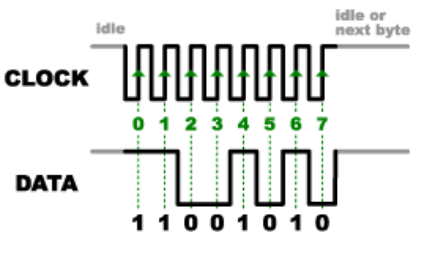
\includegraphics{figuras/sincrono.PNG}
    \end{center}
    \caption[Comunicação síncrona]{Envio de mensagem na comunicação síncrona.}
    \label{sincrono}
\end{figure}
%http://www.engineering.union.edu/~hodgsond/MER421/Winter%202015/Lectures/MER421Serial.pdf

Já na comunicação assíncrona, cada bit é enviado independentemente, respeitando o baud rate configurado, e recebido nessa mesma velocidade. Por não haver sincronismo no envio de informação, são enviados bits extras, a cada mensagem transmitida, como indicação de início de transmissão, fim de transmissão e, em alguns casos, um bit de paridade, usado para verificar a precisão da mensagem enviada.

\begin{figure}[ht]
    \begin{center}
    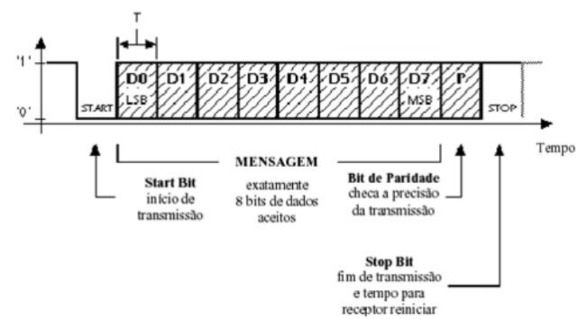
\includegraphics{figuras/assincrono.PNG}
    \end{center}
    \caption[Comunicação assíncrona]{Envio de mensagem na comunicação assíncrona.}
    \label{assincrono}
\end{figure}
%José Wilson Lima Nerys. MICROPROCESSADORES E MICROCONTROLADORES - PARTE 2 MICROCONTROLADOR 8051. 2018. 151 slides. Disponível em http://www.emc.ufg.br/~jwilson/pdf/2_Micro_Parte_2_(8051).pdf

Os microcontroladores modernos possuem capacidade de comunicação serial configurável, através da USART (receptor-transmissor síncrono e assíncrono universal), podendo assim realizar tanto a comunicação síncrona, como a assíncrona.

\subsubsection{Interrupções}

Evento que causa a suspensão temporária das atividades do microcontrolador, para que sejam realizadas rotinas específicas, de acordo com o tipo de interrupção. Após a realização da rotina de interrupção, o microcontrolador retorna ao ponto do programa em que se encontrava antes do evento. O evento causador da interrupção pode ser um fator interno ou externo. %https://docente.ifsc.edu.br/rafael.grebogi/MaterialDidatico/Mecatronica/Microcontroladores/ebook%20-%20microcontrolador%208051-%20detalhado.pdf

Existem diferentes tipos de eventos que podem causar uma interrupção em um microcontrolador, e cabe ao programador definir a ordem de prioridade entre elas:
\begin{itemize}
\item Timer - Os Timers são contadores, de 8 ou 16 bits, que incrementam a contagem de acordo com a frequência do oscilador utilizado, e geram uma interrupção no sistema ao ocorrer overflow na contagem. Os Timers podem ser configurados para contar diferentes tempos, e são normalmente utilizados como temporizadores.
\item Conversão A/D - Uma das funcionalidades da conversão A/D de microcontroladores, é a possibilidade de configurar uma interrupção do sistema quando a conversão é finalizada.
\item Comunicação serial - Dois tipos de interrupção podem ser configuradas na comunicação serial, no envio e no recebimento da mensagem. No envio, a interrupção ocorre quando o microcontrolador detecta que o buffer de envio se torna vazio. Já no recebimento, a interrupção ocorre assim que é detectado o recebimento de um byte.
\item Sinais externos - Além das interrupções apresentadas, é possível, ainda, configurar determinados pinos do microcontrolador para gerarem uma interrupção do sistema, ao receber um sinal.
\end{itemize}

\section{Programação}

Para alcançar as funcionalidades desejadas do microcontrolador, é necessário que o projetista desenvolva um programa (software) e carregue-o na memória do microcontrolador. Quando um software é feito para um fim específico, carregado em um circuito com um objetivo claro, dá-se o nome de Firmware. Um firmware é um código escrito com o intuito de ser gravado apenas uma vez no hardware, com raras modificações, normalmente em casos de correções de erros.

Cada família de microcontroladores possui um conjunto de instruções específicas a ser utilizado na sua programação. Essas instruções são escritas em Assembly, que é uma linguagem de programação que possibilita a integração das instruções do microcontrolador com funções legíveis por humanos.

Programar em assembly, porém, requer que o programador aprenda um novo conjunto de instruções para cada dispositivo diferente a ser utilizado. Para resolver esse problema, foram criados compiladores que permitem a utilização da linguagem C para a programação de microcontroladores, o que padroniza esse processo e proporciona facilidade no desenvolvimento de projetos com dispositivos distintos.



